\subsection{Objetivo 8 --- recomendações e redução de custo}

\textit{Gerar recomendações sobre o uso de Oracles em diferentes níveis como
ferramenta de análise prévia do potencial de desempenho de ensembles, considerando a
redução de custo computacional.}

A base quantitativa da recomendação é que o índice de redundância prevê a folga
\emph{antes} de treinar qualquer método de seleção:
\begin{equation}
\text{Spearman}\bigl(\dfe,\ \On{1}-\mvr\bigr) = -0.860,
\quad p = 8\times10^{-27},\quad n = 87 .
\end{equation}
Por modo: GA $-0.933$, Bagging $-0.909$, RF $-0.785$. O índice custa
$O(M^{2}n)$ sobre a matriz de acertos que já se tem.

\begin{figure}[htbp]
\centering
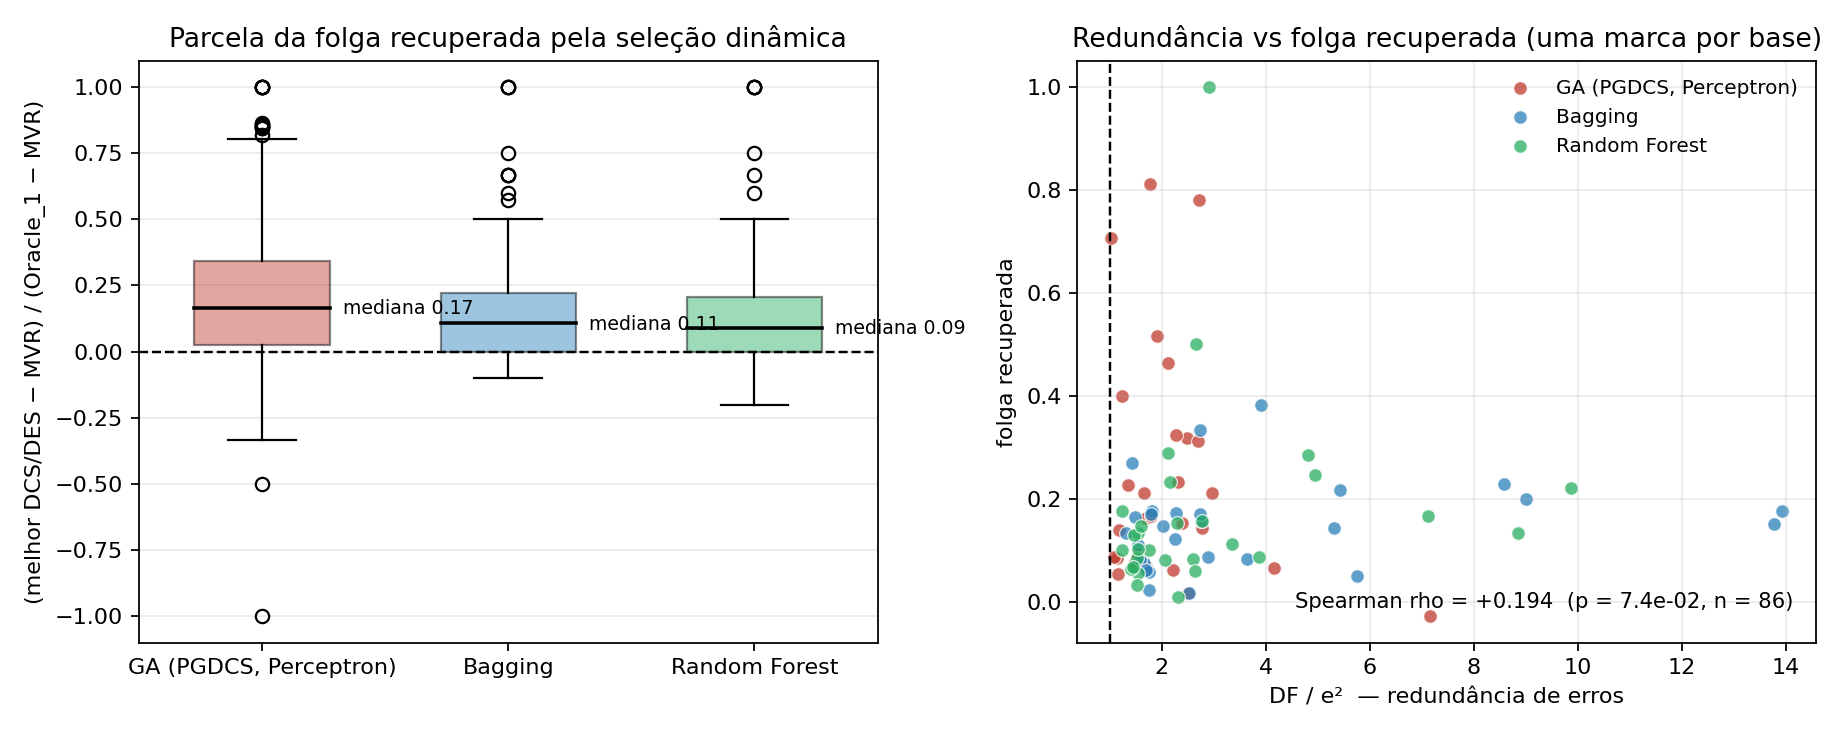
\includegraphics[width=0.95\textwidth]{figuras/fig8_recovered_gap.png}
\caption{À esquerda, a distribuição da folga recuperada por modo. À direita, a mesma
quantidade contra $\dfe$: a correlação que prevê o \emph{tamanho} da folga
não prevê a \emph{fração alcançável}.}
\end{figure}

As sete recomendações que o experimento sustenta:

\begin{enumerate}
\item \textbf{Use $\On{1}-\mvr$ como medida de potencial, não \On{1} como meta.}
O \On{1} fica entre $0.995$ e $0.998$ nos três modos e $29$ bases: não discrimina. A
folga discrimina ($0.142$ a $0.219$ entre modos; $0.017$ a $0.458$ entre bases).

\item \textbf{Não procure um \On{N} intermediário como limite realista.} $N^{*}$
fica em $N\approx M/2$ nos três modos (Friedman $p=0.40$). Reporte \On{1}, a folga e
$N^{*}$ como diagnóstico; não reporte um nível intermediário como cota.

\item \textbf{Calcule \dfe{} antes de treinar qualquer método de seleção.} Regra
operacional medida neste experimento:

\begin{center}
\begin{tabular}{lll}
\toprule
\dfe & Folga típica & Decisão \\
\midrule
$\ge 4$   & $<0.05$        & não vale DCS/DES --- o custo não se paga \\
$2$--$4$  & $0.05$--$0.15$ & marginal; só KNORA-U ou DES-P, sem esperar ganho \\
$\approx 1$ & $>0.30$      & candidato forte, sobretudo com base fraco \\
\bottomrule
\end{tabular}
\end{center}

\noindent
Extremos observados: Thyroid ($\dfe$ entre $6.96$ e $8.58$, folga $0.035$) contra P2
($\dfe = 1.02$, folga $0.458$).

\item \textbf{\dfe{} não prevê o que você vai recuperar.} Ele prevê a folga, não a
fração alcançável (por base $\rho=+0.19$, $p=0.074$; por fold $\rho=+0.02$,
$p=0.59$). São perguntas distintas. Para prever recuperação, o preditor que
funcionou é qualitativo: fronteira não-linear em baixa dimensão \emph{mais}
classificador-base fraco.

\item \textbf{Se for usar seleção dinâmica, use um método que não pode o pool.}
OLA, LCA, MCB, Rank e o melhor individual perdem de $0.044$ a $0.069$ contra o \mvr{}
nos pools de árvores, em $27$--$29$ das $29$ bases, com $p_{\text{Holm}}<0.001$.
KNORA-U é o único que supera o \mvr{} de forma sustentada em algum modo e nunca perde
em nenhum.

\item \textbf{Em pool homogêneo forte (Bagging, Random Forest) a decisão padrão é
não usar DCS/DES.} Nenhum dos $13$ fusores supera a votação majoritária de forma
significativa em nenhum dos dois modos. O melhor caso é $+0.0019$ (KNOP em Bagging),
que não sobrevive a Holm. O \mvr{} é grátis; os outros não.

\item \textbf{O custo foi medido, não estimado.} Passar de $5$ para $12$ métodos de
seleção levou o experimento de $2$h$21$ para $4$h$08$ de relógio nas mesmas $29$
bases $\times$ $10$ folds $\times$ $3$ modos --- fator $1.76\times$. Combinado com a
recomendação 6: o custo marginal de DCS/DES é da ordem do custo de gerar os pools, e
num pool de árvores ele compra zero.
\end{enumerate}
